\scanpage{50}
\deleted{\unsure{Autre façon}}

Ceci ne nous a pas donné de façon très explicite de classifier les ``courbes \inserted{\unsure{simples}} de genre $0$'' sur $S$, munies d'une section et d'une trisection non ramifiée, disjointes
\margin{\figure{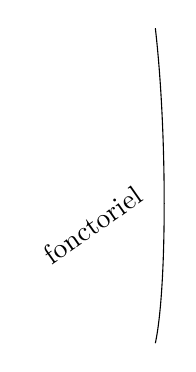
\begin{tikzpicture}[x=1cm,y=1cm]\node[rotate=35] at (-.8,0) {fonctoriel};\draw (0,2.5) .. controls (0.15,1.2) and (.15,-.8) .. (0,-1.5);\end{tikzpicture}}}
[\deleted{$\unsure{X}$} $=$ \unsure{revêtement} $\unsure{\mathfrak S_3}$ \unsure{non} ramifié \inserted{$S'$} de groupe $\mathfrak S_3$ de $S$, avec une section \deleted{de} de
\[
\deleted{\unsure{X\simeq P^1_S\times_{(S,\mathfrak S_3)}}}\quad S'\times_{(S,\mathfrak S_3)}\unsure{\mathbf P|P}^1_S
\]
\inserted{$t$ disjoint de $0,1,\infty$,} invariant par le groupe $\mathfrak S_3$, i.e. \deleted{une section}
\[
t\in\Gamma(S',\underline O_{S'}),
\]
inversible et telle que $t-1$ soit inversible, et satisfaisant à
\[
\sigma.t=\deleted{\unsure{\varphi}}\unsure{\bar\sigma}(t)\qquad\sigma\in\mathfrak S_3
\]
i.e.
\[
\begin{cases}\lambda t=\dfrac1t\\\mu t=1-t\end{cases}
\]
\margin{\diagram{\begin{tikzcd}X\arrow[d]&P^1_{S'}\arrow[l]\arrow[d]\\S&S'\arrow[l,"\mathfrak S_3"']\end{tikzcd}}}
\figure{\begin{tikzpicture}\draw (0,1.2) to[bend right=8] (0,.2)--(.25,0);\end{tikzpicture}}

\margin{\uuline{non} \uline{fonctoriel}}
\uline{Exemple} $S=\operatorname{Spec}(O)$, $O$ anneau local \uline{complet} à corps résiduel $\mathrm{alg.}^{\mathrm t}$ clos \deleted{\unsure{(car. $\ne2,3$)}} \inserted{(de car. $\ne2,3$)}.

Alors \deleted{$\unsure{X\simeq P^1_S}$} $\pi_1(S)=0$, donc la situation équivaut, \inserted{[\unsure{Donn. non canoniq.|Donn. non canonique} \unsure{par} \unsure{quoi}]} à la donnée d'un $t\in O^*$ tel que \deleted{$\unsure{t(t-1)\in\mathbb Z}$} $t(t-1)\in O^*$, étant entendu que $t,t'$ donnent des \unsure{représ.} isomorphes \deleted{\unsure{si et}} s. s. s. $t'$ est de la forme \inserted{$\bar\sigma(t)\quad\sigma\in\mathfrak S_3$.}
\mspage{49}
